\section{SimCADO -- the Python package for simulating MICADO observations}
\label{sec:scope}

\subsection{Motivation and Scope}
\label{subsec:motivation_scope}

The scientific return of instruments like the ELT and MICADO is the primary reason for building such complex pieces of machinery.
Knowing in advance what the capabilities of an instrument will be, and preferably knowing just how well the instrument will perform for different configurations is invaluable during the design phase.
Furthermore, MICADO and the other ELT instruments (e.g.\ HARMONI, \citealt{harmoni}; METIS, \citealt{metis}; etc.) are being built by trans-national consortia, with many members from different institutes in different countries.
As such the nodes in the consortia enjoy a certain level of geographic displacement.
Each node in the consortia therefore often defaults to generating their own simulated data for the task to which they have been assigned.
Additionally, the end users of the instrument also want to know how the instrument will behave and how useful it will be for their personal scientific projects well in advance so that they may prepare for when the instrument becomes available.
All of these points can be considered true for almost all large instrument projects in modern day science -- hence why there has been a very concerted effort by the scientific community, and very notably by the astronomical community to develop full scope instrument data simulators for major projects (see e.g. HSIM for ELT/HARMONI, \citealt{hsim}; the ELT/METIS simulator, \citealt{metissim}; PhoSim for the LSST, \citealt{phosim}; TOAD for 4MOST, \citealt{toad}; WebbPSF for JWST, \citealt{poppy}; IRIS Data Simulator for TMT, \citealt{irissim}; etc.).


\subsection{The SimCADO target users}
\label{subsec:users}

We have developed SimCADO for use primarily within the MICADO consortium, but also for interested external parties.
SimCADO's main strength is that it gives all members of the consortium a common tool to generate simulated data for their assigned tasks.
We see the following use cases for SimCADO:

\paragraph{The science team:} During the current design phase the science team members are running feasibility studies to determine which science cases are the biggest drivers for the design of the instrument. By using a common tool to generate simulated images, the science team, and those using the findings of the science team to make design decisions, can be confident that the results are all consistent. 

\paragraph{The astronomy community at large:} Although first-light for the ELT is slated for 2024, preparation work needs to begin well in advance so that the astronomical community can ``hit the ground running'' once the ELT and MICADO are online. Many of the ideas that will be tested post-2024 will need to be developed over the coming years. It is therefore important that the astronomical community have a tool that enables new ideas to be thoroughly tested, and where necessary, preparation observations to be conducted, before applying for time with MICADO. SimCADO can help test the feasibility of observations for new ideas.

\paragraph{MICADO and ESO data flow teams:} In order to create a reliable set of reduced data products which are available from the beginning of operations, the data reduction pipeline must be developed before the first data are collected. Development of the pipelines can happen concurrently to the develpment of the instruments, however without a telescope there is little that can be done to validate these pipelines before the commissioning of the telescope and instruments. SimCADO takes into account all processes that affect the incoming light as is travels from the source to the detector. As such SimCADO can substitute for the ELT and MICADO by producing so-called ``dirty'' raw detector frames for the reduction pipeline, thus allowing the pipelines to be validated well in advance of the commissioning phase.

\paragraph{Observation preparation software:} Given the capabilities and expense of the ELT/MICADO system, observation time will be costly and in high demand. Therefore it is prudent to optimise observations to maximise the scientific output from any time on-sky. Currently, exposure time calculators are provided to assist in observation preparation. However, given the myriad celestial environments encountered during observations, single numbers based on look-up tables are often not enough to accurately predict exposure times. For the ELT/MICADO system, using SimCADO together with the preparation software will allow the user to not only determine the required exposure time, but also to visualise and assess the effect of surrounding objects on the detectability of the target object. This should help to reduce the number of non-detections during actual observations and increase the scientific output of the MICADO and the ELT.

\paragraph{The data archive:} The ability to produce simulated data also allows the development of a data archive to proceed prior to the availability of real data. SimCADO images will be used to help define the data products offered by MICADO and the method of storage and retrieval well before the instrument generates any images of its own accord.
  
\paragraph{Instrument design team:} SimCADO relies heavily on input from the different consortium work packages in order to produce images representative of the whole instrument. This in turn means that, by providing multiple sets of input data for a specific component in the optical train, a work package can use SimCADO to test the effect of different component designs on the final image quality. By using a standard set of use cases and weighting the importance of each aspect of the various science cases, trade-off analyses can be conducted. It should however be noted that due to its scope and design, SimCADO is not meant to replace ray tracing programs such as ZEMAX (see Sect.~\ref{ssec:IDS}). For such cases the SimCADO output should only be used to guide more realistic physics-based simulations, e.g.\ with ZEMAX, before making any final decisions.
  
\paragraph{The MAORY consortium:} MICADO will be the first and main beneficiary of the MAORY AO module \citep{maory}. Consequently the development of the MAORY module is inextricably linked to MICADO. Design choices made in the MAORY consortium will have a direct impact on the quality of the science that MICADO will be able to produce. By using SimCADO, members of the MAORY consortium will also be able to see directly how these design choices will affect MICADO observations.
  

\subsection{SimCADO as an Instrument Data Simulator}
\label{subsec:IDS}

First and foremost SimCADO was conceived as an instrument data simulator (IDS), not an end-to-end (E2E) simulator. An IDS differs from an E2E simulator in the following way: an E2E simulator models the interactions between each object and each element in the optical train with the incoming photons in a physically realistic manner, i.e.\ taking into account the physical interactions between photons and computer representations of physical objects along the optical train (see photon-tracing in PhoSim for the LSST: \citealt{phosim}). An IDS, on the other hand, turns the effects of each element in the optical train into mathematical operators, which are then applied to an input ``image'' (a 2D/3D representation of the sky). IDSs require much less computation power and are therefore much better suited for quick, personalised simulations and prototyping. However, this comes at the cost of flexibility. E2E simulations can create images for any physical configuration of the optical train, as long as a physical model of all components exist in memory. IDSs only generate output for a certain configuration if data (often originally created by an E2E simulation) already exists and can be converted into a series of mathematical operators. A good example is the case of the PSF. Given a point source with a certain brightness, the PSF will appear on the focal plane of an E2E simulation by only supplying a model of the physical objects along the light's path (spiders, mirrors, pupil stops, etc.). An E2E simulator needs only the values pertaining to the physical positions and dimensions of these objects. An IDS on the other hand is able to project a PSF onto the focal plane because a mathematical description (either a 2D image array or a 2D function) of that PSF has been supplied. The IDS then convolves this description with one or many point sources. Regardless of how the optical train changes, unless this mathematical description has been updated from another source (i.e.\ output from a separate E2E simulator) the IDS images will continue to display the same PSF.

The main advantage of developing and using an instrument data simulator lies in its speed and ease of use. Because IDSs rely on the results of other simulations, IDS simulations are many orders of magnitude faster than those conducted with E2E simulators. Our main goal with SimCADO was to provide a tool that gives the casual user the ability to simulate images for MICADO in a matter of minutes on their own laptop. Such an approach is advantageous to both the user and the developer when compared to the alternative model: the user must submit a simulation request to a dedicated ``simulations'' team. With SimCADO running on the user's laptop, both the time the user must wait for results and the work load of the simulations team are drastically reduced. This in turn allows the simulations team to direct their efforts towards improving the software and keeping the instrument configuration up to date.

Further justification for concentrating our efforts on an IDS rather than an E2E package comes from the fact that for the majority of cases (excluding those from the design team), the optical train stays exactly the same. Therefore there is no need to re-simulate from scratch each and every photon interaction (as an E2E simulator would do) every time a simulation is run.


\section{The physical effects modelled by SimCADO}
\label{sec:simcado}

SimCADO takes into account effects for all optics elements between the light source and the detector. This includes the atmosphere, the telescope, the instrument, and the detector array. We have designed SimCADO in such a way as to allow any optical train to be modelled, providing all the relevant data is available\footnote{We have also created configuration packages for the HST+WFC3 system and the VLT/HAWK-I systems.} The default configuration is for the ELT/MICADO optical train. For testing purposes we have configured SimCADO to reproduce the effects of the VLT/HAWK-I optical train (see Sect.\ \ref{sec:hawki}). In this section we describe the effects of the optical elements that the current version (0.4) of SimCADO takes into account. 

For a full description and discussion of the internal workings of the SimCADO package, the reader is directed to the paper by \citet{leschinski2016} and to the online SimCADO documentation.\footnote{\url{http://www.univie.ac.at/simcado}} 


\subsection{Atmosphere}

\begin{figure*}

    \centering
    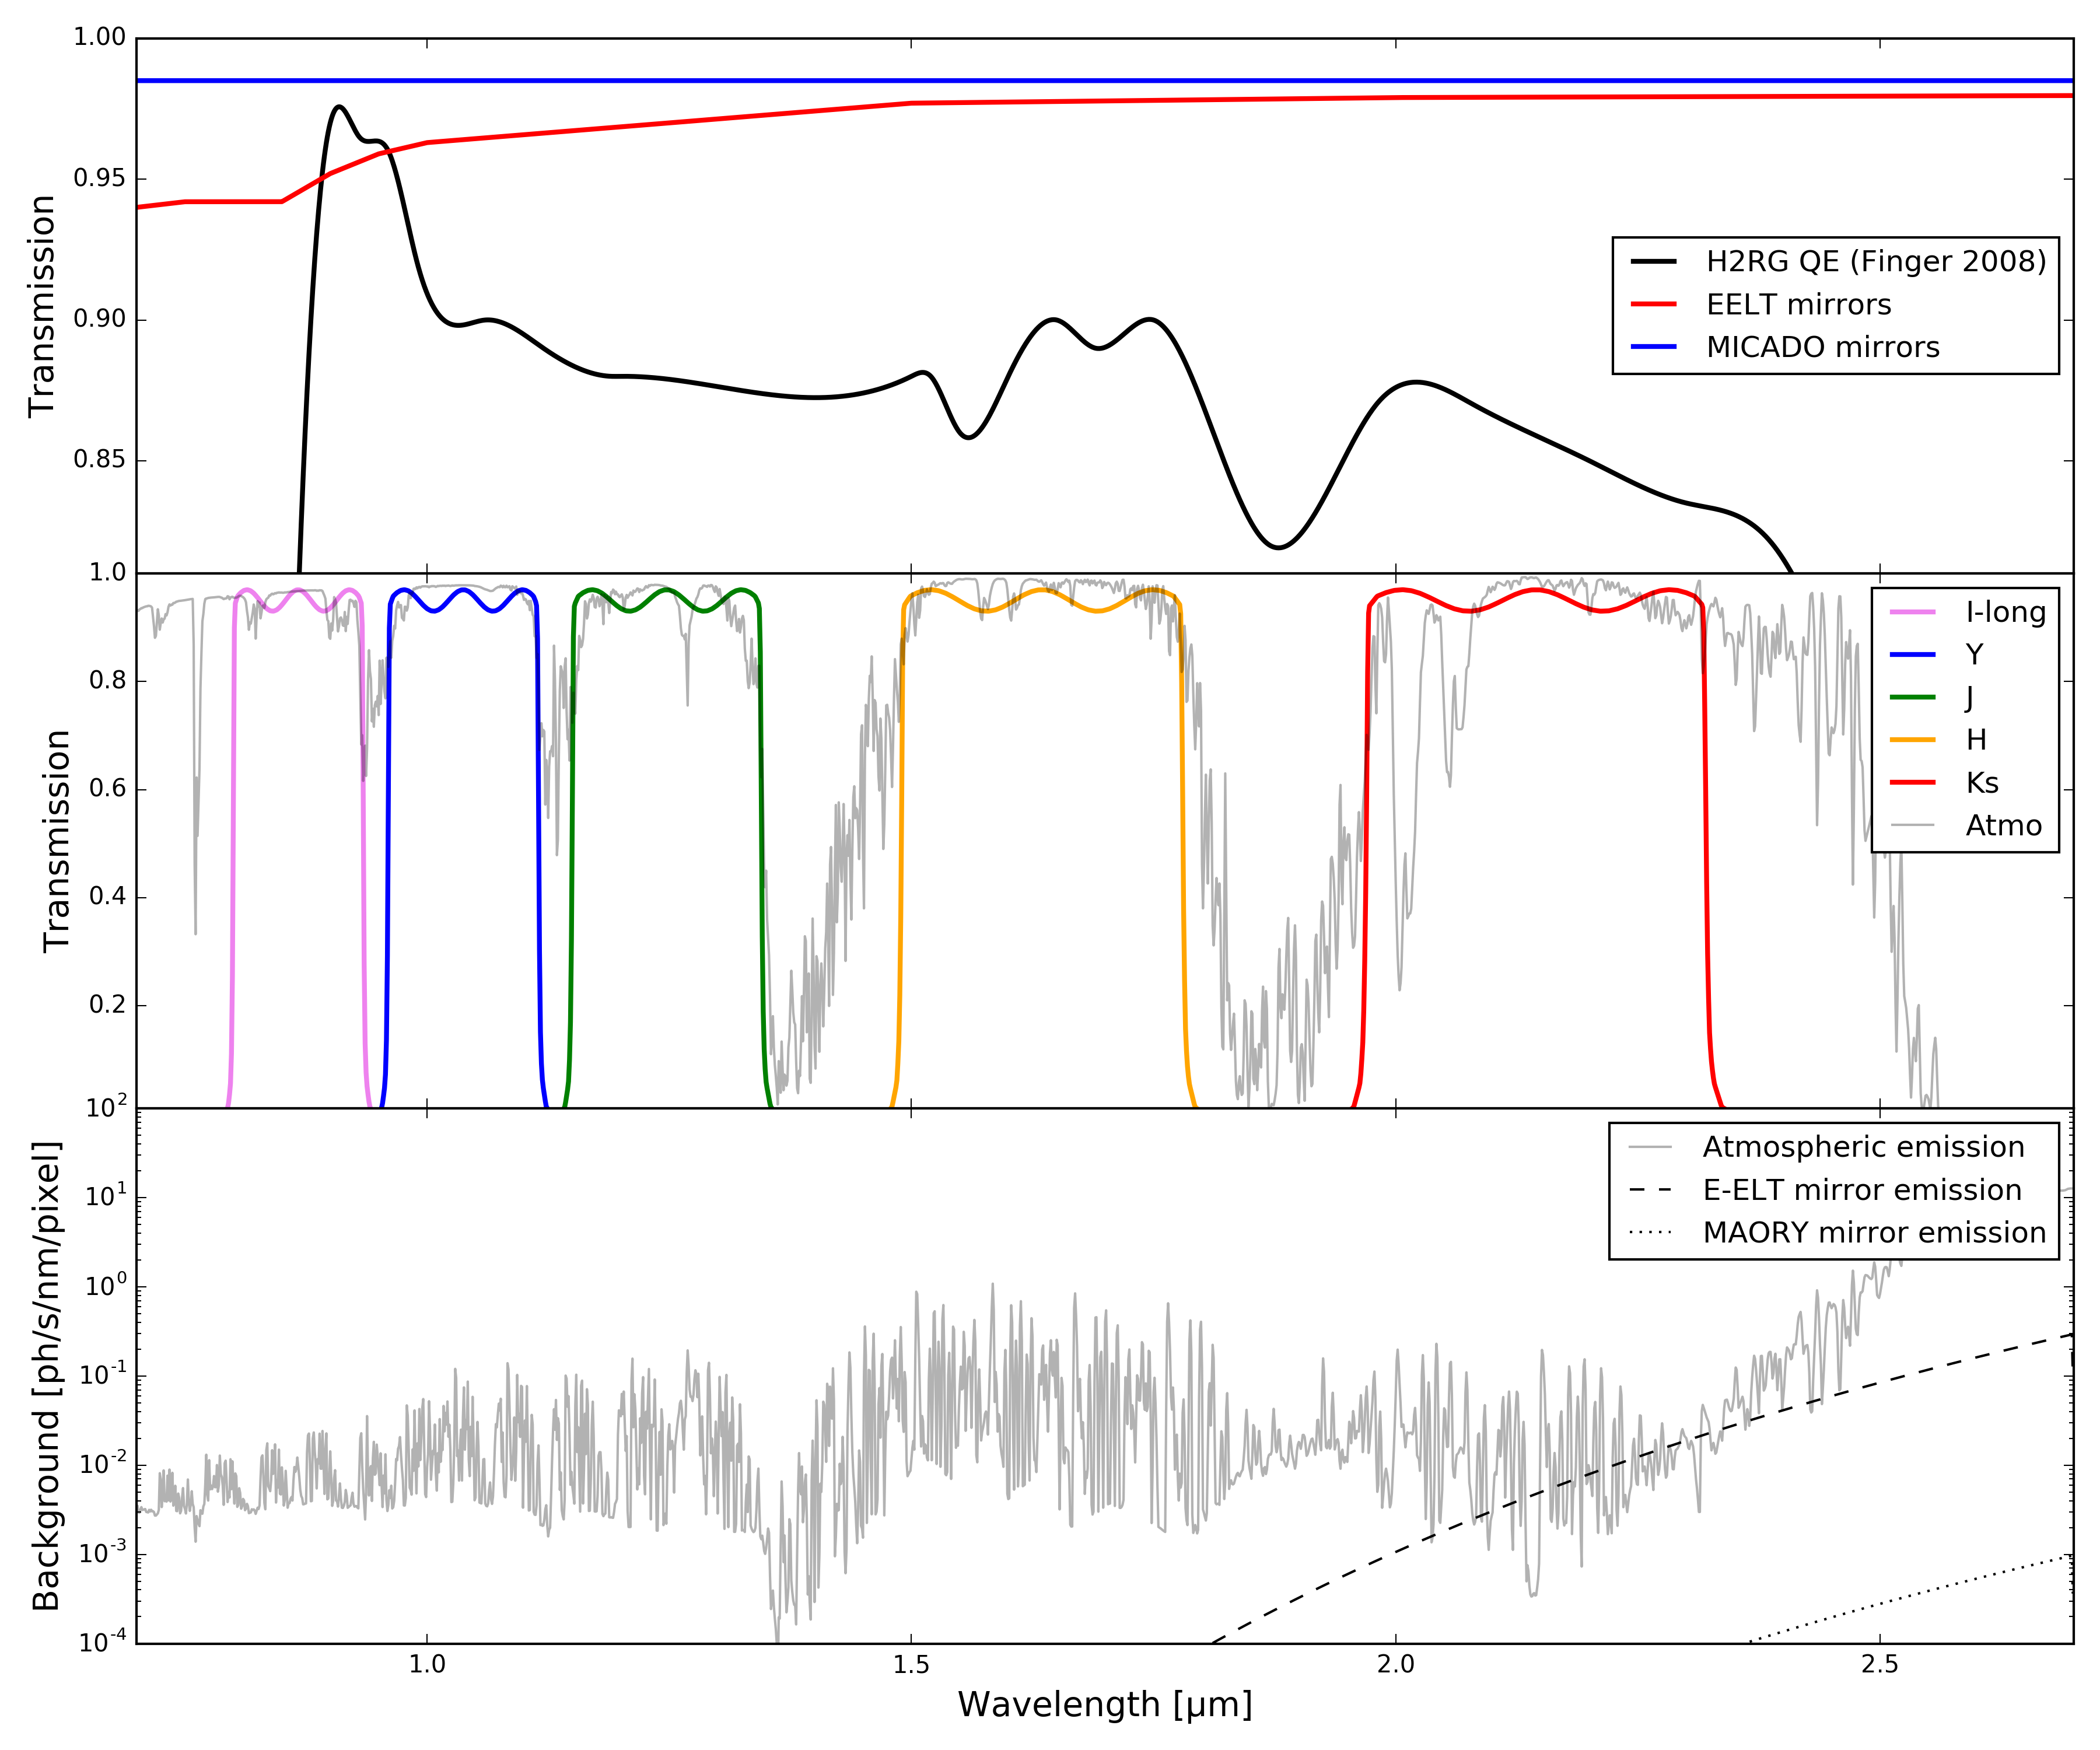
\includegraphics[width=\textwidth]{images/fig1_spectra}

    \caption{Default transmission and emission curves used by SimCADO. Top: The mirror transmission curves for both the ELT and MICADO plotted together with the quantum efficiency (QE) curve for the HAWAII 2RG detectors. The ELT will use a AgAl mirror coating with a MgF\textsubscript{2} protective layer \citep{boccas06} while the 14~MICADO mirrors will be gold coated \citep{micado2016}. SimCADO uses the QE curve for the H2RG detectors because this information for the H4RG detector is not currently available to the public. As soon as the QE curve for the 4k detectors becomes available, the SimCADO defaults will be updated. Middle: A selection of broadband filters for MICADO (IYJHKs) based on theoretical filter properties. SimCADO ships with a collection of curves for the filters currently foreseen for use in MICADO. The atmospheric transmission curve used by SimCADO was generated by the skycalc tool \citep{skycalc1, skycalc2} and can be adjusted for zenith distance. Bottom: the photon background flux per MICADO wide-field mode pixel (i.e.\ 4\,mas) coming from the atmosphere and from the ELT and MAORY mirror grey-body emission. The units are photons per second per nanometer calculated for the full area of the ELT's mirrors. The sky background emission spectrum was generated using the skycalc tool with the default parameters. The ELT mirror emission is for an ambient dome temperature of 0~degrees Celsius and combines the emission from all five of the ELT's mirrors. The MAORY mirror emission is assuming warm optics at the dome temperature and the optical train as detailed by \citet{maory} and \citet{maory2016}. The total area of the MAORY mirrors is taken to be $3.4\,\mathrm{m}^2$. }
    
    \label{fig:1_spectra}
    
\end{figure*}


\paragraph{Transmission and Emission:} 
The SkyCalc tool\footnote{\url{https://www.eso.org/observing/etc/bin/gen/form?INS.MODE=swspectr+INS.NAME=SKYCALC}} \citep{skycalc1, skycalc2} provides accurate spectral models of the atmospheric transmission and emission (see Fig.~\ref{fig:1_spectra} for the transmission and emission curves). For SimCADO we have taken the default model, which uses atmospheric conditions averaged over the whole year and a unity airmass. In a future release we hope to include the functionality to query the SkyCalc server directly from within SimCADO. However until such time, if the user is interested in investigating the effects of different atmospheric conditions on the resulting detector output, SimCADO accepts ASCII text files generated by the online SkyCalc tool as input for simulation runs.

As an alternative to using the default spectral energy distribution provided by SkyCalc, the user may instruct SimCADO to use a certain sky background emission for a given broadband magnitude in mag/arcsec$^2$. 
%The number of photons are calculated from a spectrum of Vega multiplied by the transmission curve for the given broadband filter and scaled according to the user's sky background surface brightness.

\paragraph{Atmospheric diffraction:} 
For effects that act along all three relevant simulation dimensions ($x$, $y$, $\lambda$) SimCADO uses an adaptive layered approach. Briefly this means that SimCADO determines how separated in spectral space two individual images can be before a noticeable spatial shift between two adjoining layers occurs. This parameter can be set in the SimCADO configuration file. By default a new spectral bin is created once the shift due to the atmospheric dispersion is greater than one pixel (i.e.\ 4\,mas and 1.5\,mas in the wide-field and zoom modes, respectively). The spatial shifts induced by the atmosphere are calculated according to the formulae from \citet{stone1996} and from the review by Pedraz\footnote{\url{http://www.caha.es/newsletter/news03b/pedraz/newslet.html}}. In order to avoid unnecessarily increasing the computational workload, any shifts induced by the atmospheric dispersion are inversely scaled according to the performance parameter for the atmospheric dispersion corrector (ADC). By by default this is set to 100\,\% -- i.e.\ no atmospheric dispersion is included.

\paragraph{PSF variability}: 
SimCADO does not compute the atmospheric point spread function itself based in atmospheric parameters. Instead it requires a PSF to be provided, either by the other teams working in conjuction with the MICADO consortium (i.e.\ the SCAO and MCAO simulation teams) or by the user. PSFs will be discussed in greater detail in Sect.~\ref{sec:eelt_psfs}; however, it is worth mentioning here that SimCADO provides a series of functions for generating ``ELT''-like PSFs based on the POPPY PSF simulation package \citep{poppy}. The function \verb+simcado.psf.poppy_ao_psf()+ allows the user to specify the level to which the seeing halo is added to an ideal diffraction limited PSF, thus allowing the user to create PSFs for different seeing conditions.

Currently SimCADO does not automatically include time variability in the PSF or in the atmospheric parameters. However, SimCADO's implementation in Python allows the user to script many different simulation configurations, thus providing the functionality to implement temporally varying atmospheric conditions. An automated method for doing this is foreseen for later releases of SimCADO.


\subsection{The ELT}
\label{sec:eelt_psfs}

\begin{figure*}

    \centering
    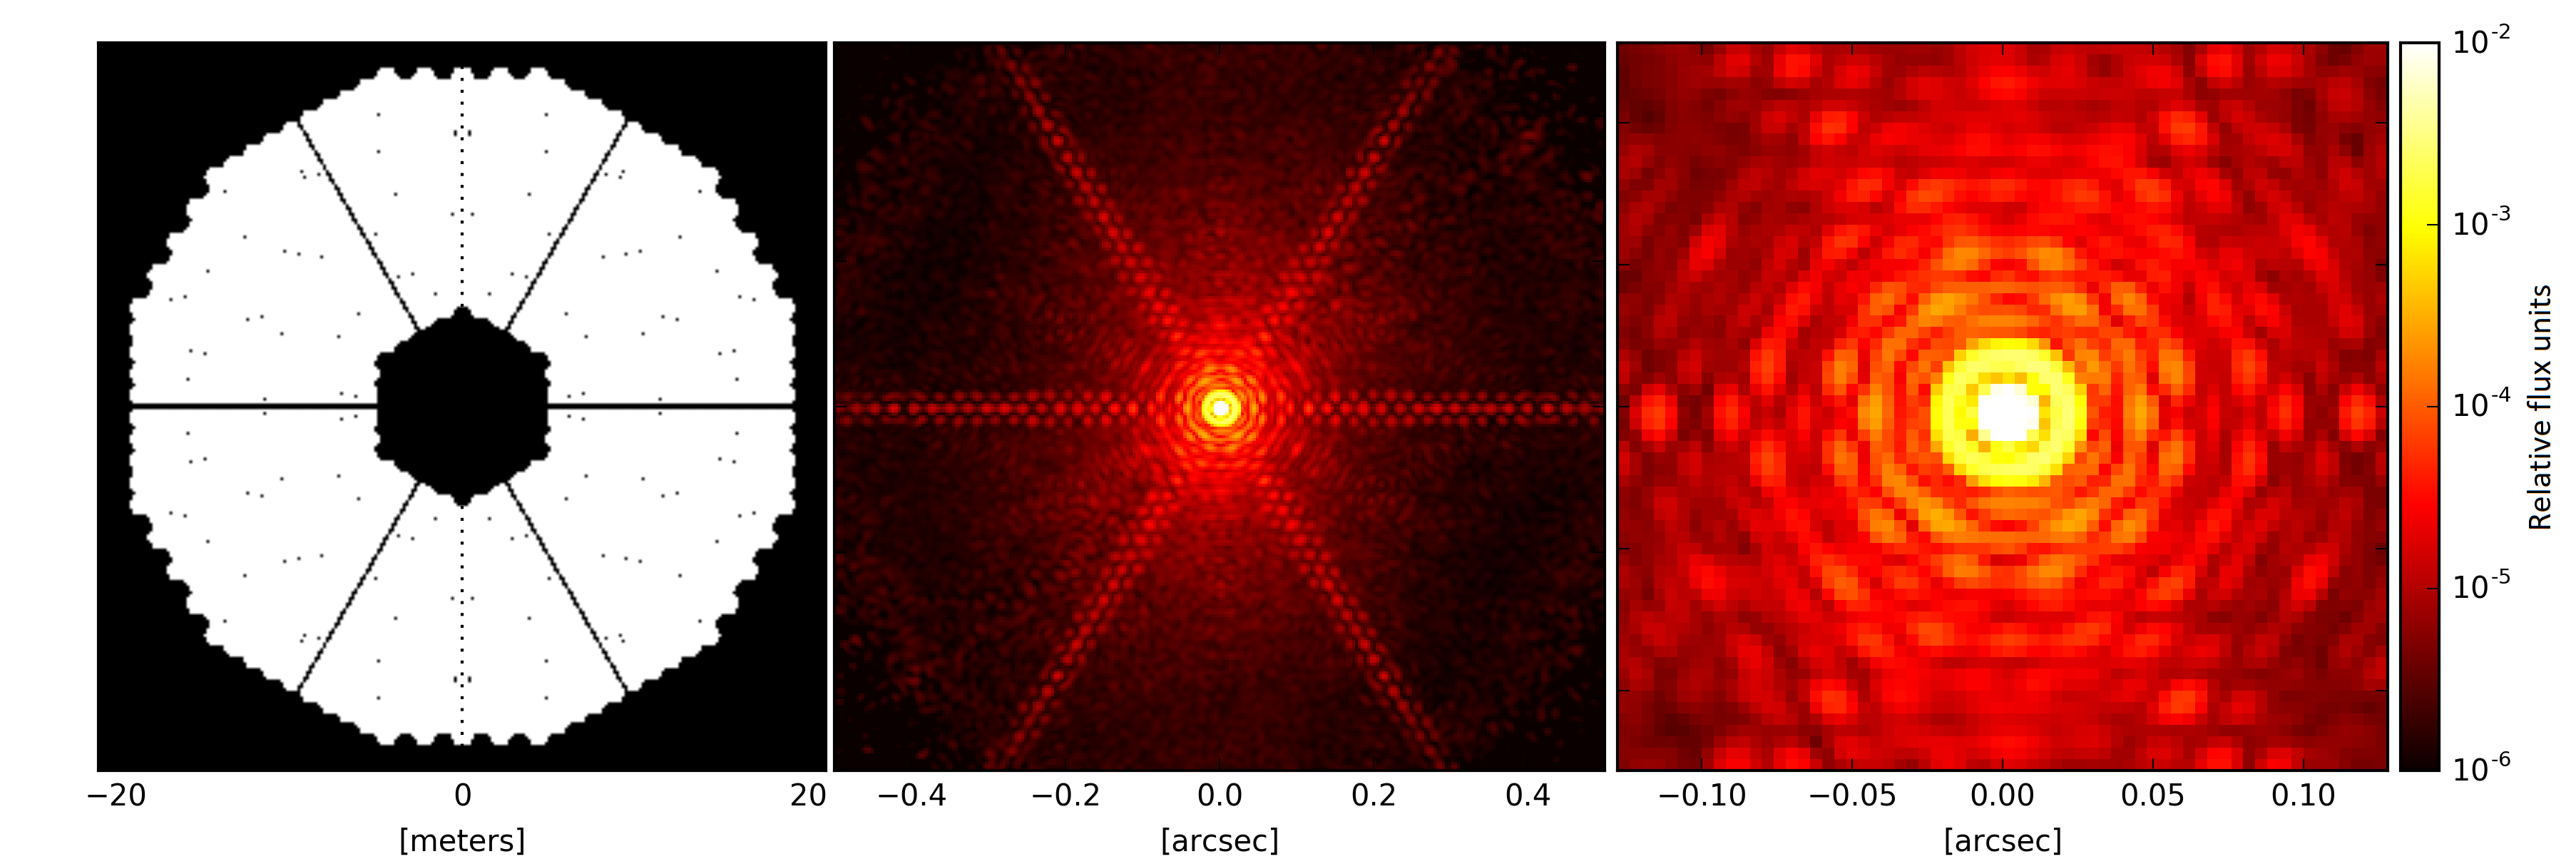
\includegraphics[width=\textwidth]{images/fig2_eelt_psfs_SR50}

    \caption{Left: the ELT pupil with the full mirror configuration, not taking into account any circular obscuration in subsequent pupil planes. Middle: the current SCAO PSF used by SimCADO as developed by \citet{clenet2013}. The PSF has a Strehl Ratio of 68\,\% in the Ks band over a $4\arcsec$ FoV. The effects of a segmented mirror on the diffraction spikes are clearly visible. Right: a cutout of the central $0.25\arcsec$ of the PSFs. The effect of the segmented mirror is also present in the structure of the Airy rings around the core of the PSF.}

    \label{fig:2_elt_psfs}

\end{figure*}


\paragraph{Point Spread Function:} Being an IDS, SimCADO does not need to know how the PSF is generated or what happened to it before the instrument focal plane. All SimCADO needs is the total (wavelength dependent) effect of the whole optical train on the spatial distribution of light on the focal plane. How the atmosphere deforms the PSF and how the AO modules correct for this are outside the scope of SimCADO. Only the net effect of the two counteracting operations are important for simulations.

Currently the two adaptive optics (AO) modes that will be offered with MICADO are: 
\begin{itemize}

    \item single conjugate \citep[SCAO,][]{clenet2016}, which will provide diffraction-limited imaging with Strehl ratios of $>60\,$\% in Ks-band in the centre of the field of view.
    \item multi-conjugate (MCAO) in conjunction with the MAORY module, which will provide diffraction-limited imaging of the full MICADO field of view with Strehl ratios between 30\,\% and 50\,\% in Ks band \citep{maory2016}

\end{itemize}

Currently, SimCADO only provides a SCAO PSF from the AO simulation efforts of \citet[obtained via private communication]{clenet2015}. MCAO PSFs will be included as soon as the MAORY consortium releases them for public use. Additionally SimCADO also provides functionality to generate lower fidelity PSFs using an analytical model. This model is not as accurate as the E2E simulations but it does allow the user to conduct comparative studies. For example, the user can investigate how different Strehl ratios will affect the results for a certain science case. The analytical PSF is generated by summing two weighted PSFs, a diffraction-limited PSF and a seeing-limited PSF, according to the equation:

\begin{equation}
   \mathrm{PSF}_{\mathrm{Analytical}} = \mathrm{SR} \times \mathrm{PSF}_{\mathrm{Diffraction}} + (1 - \mathrm{SR}) \times \mathrm{PSF}_{\mathrm{Seeing}}, 
   \label{eq:strehl_ratio}
\end{equation}

where SR is the desired Strehl ratio, PSF$_{\mathrm{Diffraction}}$ is the diffraction-limited PSF generated by the POPPY package \citep{poppy} for a 39\,m diameter segmented mirror with six support beams for the secondary mirror (see Fig.~\ref{fig:2_elt_psfs}), and PSF$_{\mathrm{Seeing}}$ is a PSF following a Moffat profile with a full width half maximum (FWHM) corresponding to the seeing limit of the observations. For the seeing-limited PSF, SimCADO uses a FWHM  of $0.8\arcsec$ by default. The default Strehl ratio for the analytical PSF is set to the Strehl ratio that MAORY is required to provide, i.e.\ 30\,\% in K band and 12\,\% in J band \citep{maory2016}. Currently, SimCADO does not vary the shape of the PSF over the field, as would be consistent with AO observations. We are however developing this functionality for a future release


\paragraph{Transmission and emission:} SimCADO uses the reflectivity curve provided by the ESO Data Reference Mission (DRM) for the ELT\footnote{\url{https://www.eso.org/sci/facilities/eelt/science/drm/}} for an aluminium-silver mirror coating with a magnesium flouride protective layer (AgAl-MgF\textsubscript{2}). This is currently the preferred mirror coating for all five of the ELT mirrors. For comparison SimCADO also provides the transmission curve for a pure aluminium coating (as used at the VLT). The reflectivity in the near infrared regime is almost constant at $\sim 98\,\%$.

The grey-body emission  for the ELT is calculated by looping through each of the mirrors designated in the optical design. The emitted flux is calculated by considering the area, emissivity and temperature of each mirror. Transmission losses for each mirrors grey-body flux due to the subsequent mirrors in the optical path are also taken into account in the loop.

%The grey-body emission for the ELT is calculated by assuming all emission is coming from a single surface with the combined area of all five mirrors ($\sim 1030\,\mathrm{m}^2$) and at a temperature of 0~degrees Celsius. This light is subject to the transmission losses of all five ELT mirrors. While this is not a completely correct representation of what happens to the grey-body emission -- light from M1 is subject to reflectivity losses from 4 mirrors, while there is no loss of emitted light from M5 due to ELT surfaces -- because of the shear size of M1 ($\sim$980m$^2$) the difference in total grey-body light from the five ELT mirrors is $<0.15\%$.  \occomment{But this has been implemented correctly a long time ago!} This source of uncertainty is far outweighed by the uncertainty in the assumed temperature of the mirrors. The increase in computation speed by only using one characteristic transmission curve for the grey-body emission is noticeable and justifies this approximation.


\paragraph{Wavelength independent spatial effects:} Effects related to unwanted movements of the telescope are also built into SimCADO. Wind jitter and vibrations due to the cooling equipment introduce a further blurring term into the image. This can be modelled by convolving the final focal plane image with a 2D Gaussian distribution. The FWHM of the Gaussian is a function of the frequency spectra and the strengths of both the vibrations and the wind. At this stage we have assumed that the ELT's vibration damping mechanisms will remove the vast majority of vibrations. As such default vibrations in SimCADO are modelled with a 2D Gaussian with a FWHM of $0.001\arcsec$, thus removing this effect from the default simulations.

SimCADO provides the functionality to simulate the smear introduced by sub-optimal mechanical performance of the ELT's tracking system. However a quick back-of-the-envelope calculation shows that the update frequency of the ELT's stepper motors needs to be on the order of $10-100\,\mathrm{kHz}$ if the sky is to move less than a MICADO pixel length between updates. This is well within the scope of modern day stepper motor technology and so by default SimCADO assumes that the ELT's tracking system will not cause noticeable image smearing. 


\subsection{MICADO}
\label{ssec:MICADO}
We have developed SimCADO during the preliminary design phase of MICADO. The default configuration for SimCADO is continually updated to reflect the most recent design of the instrument. Values presented in this subsection are correct at the time of publication, but need not be identical to those in the most recent version of the SimCADO package. See \citet{micado2016} for the MICADO design at the time of writing.

\paragraph{Transmission:} SimCADO takes into account all optical surfaces along the instrument optical train including: the cryostat entrance window (4~surfaces), the internal fold mirrors, the atmospheric dispersion corrector (4~prisms, 8~surfaces), the zoom optics, the filters (2~surfaces) and the pupil placeholders. Additional surfaces needed for the spectroscopy mode include the entrance slit and the grisms. These will described in a companion paper on the SimCADO spectroscopy mode. 

% Include default filter information ?? Entrance window etc?

Currently by default all the mirrors are assumed to be coated with gold with a reflectivity of 98.5\,\% across the whole spectral range. The filter curves shown in Fig.~\ref{fig:1_spectra} are theoretical predictions for the MICADO filters (R. Davies, private communications). The real filters will not have such a clean oscillatory transmission structure. Additionally SimCADO ships with all generic visual and NIR broadband filters (UBVRIzYJHKKs) and a series of common narrow band filters for NIR observations, taken from the Spanish virtual observatory database\footnote{\url{http://svo2.cab.inta-csic.es/theory/fps3/index.php?mode=browse}}. The user is also able to direct SimCADO to use any filter curve for which they have an ASCII file containing wavelength and transmission values by using the \verb+TransmissionCurve+ object. See the SimCADO documentation for more information. 


\begin{table}

    \centering
    \caption{The root-mean-square wavefront error expected for each surface in the MICADO optical train. The total wavefront error is expected to be on the order of 76\,nm, which translates to a decrease in PSF peak strength of $\sim 5\,\%$ at $2.2\,\micron$ $\sim14\,\%$ at $1.25\,\micron$ (R. Davies, private communication)}
     \begin{tabular}{c c c c}
        \hline\hline
        Wavefront error &  Surfaces  &   Material  &  Optical element \\
         rms [nm]       &            &             &                  \\
        \hline
        20              &     11     &       gold  &      Mirror \\
        10              &      4     &       glass &      Entrance window \\
        10              &      2     &       glass &      Filter \\
        10              &     8      &       glass &      ADC\\
        \hline
    \end{tabular}
    \label{tab:wfe_individual}

\end{table}


\paragraph{Non Common Path Aberrations (NCPAs):} The default PSFs do not take into account the NCPAs due to the difference in optical path to the wave-front sensors and to the detector array. Characterising the MICADO NCPAs is still an active topic. We will include both the spatial and spectral effects of the NCPAs in a later release of SimCADO once a model exists to describe the spatial effect. In the meantime we are able to use wave-front error budgets to determine an approximate wavelength-dependent effective transmission loss, $\Delta f_{\mathrm{peak}}$, based on the exponential form of the Strehl ratio \citep{mahajan1991}:
%wavelength dependent reduction in the peak intensity, , of the PSF due to the NCPAs according to Eq.~(\ref{eq:wfe}):

\begin{equation}
    \Delta f_{\mathrm{peak}} = \mathrm{e}^{-(2\pi \mathrm{WFE}_{\mathrm{total}}/\lambda)^2},
    \label{eq:wfe}
\end{equation}

where $\mathrm{WFE}_{\mathrm{total}}$ is the combined r.m.s. wavefront error expected for all surfaces along the MICADO optical path and $\lambda$ is the wavelength at which the observations are conducted. Table~\ref{tab:wfe_individual} details the individual wavefront errors that SimCADO uses to calculate $\mathrm{WFE}_{\mathrm{total}}$. The total wave front error is expected to be on the order of 76\,nm which translates to a decrease in PSF peak strength of $\sim 5\,\%$ at $2.2\,\micron$, and $\sim 14\,\%$ at $1.25\,\micron$ (R. Davies, private communication).


\paragraph{Atmospheric Dispersion Corrector (ADC):} Like the PSF, the effect of atmospheric dispersion is visible in all three instrumental dimensions ($x$, $y$, $\lambda$). In order to simulate this effect SimCADO creates an image for each one of a series of spectral bins within the filter wavelength range (see \citealt{leschinski2016} for a detailed description of how SimCADO does this). The bin width is chosen in such a way that the elongation induced by the atmospheric dispersion is never greater than one pixel (i.e.\ 4\,mas in wide field mode, or 1.5\,mas in zoom mode). If the ADC is working perfectly then the atmospheric dispersion is completely removed and the spectral bin width is equal to the full width of the filter. If the ADC is turned off, the relative shift of an image over the full J-band is around $0.19\arcsec$, or almost 50~wide-field pixels, at a zenith distance of 60~degrees. To maintain a relative offset between images of less than a single pixel, SimCADO must generate images for each of the almost 50~wavelength bins. Each image is offset relative to the image of the reddest bin. By stacking all the images (including offsets) on the detector plane the dispersion caused by the atmosphere can be reproduced in the final output image. By default SimCADO assumes that the ADC achieves its design specification of no more than a 1\,mas dispersion residual and so does not need to introduce any extra image slices. The functionality is nevertheless included in SimCADO.

\paragraph{Derotator:} A perfectly functioning derotator is essential for maintaining the astrometric accuracy of sources near the edges of the detector plane. Similar to the ADC we have implemented the effect of a less-than-perfect derotation by combining a series of image slices for which the shift at the edge of the detector array is less than one pixel. However as the sky rotation is a purely spatial effect, the image slices are generated for temporal bins (i.e.\ a series of short ``exposures''), as opposed to the spectral bins for the ADC (again, see \citealt{leschinski2016} for further details). By default, SimCADO assumes perfect derotation, but as always the defaults will be updated as soon as more information becomes available.

\paragraph{Instrumental Distortion:} Another effect that is important for accurate astrometric measurements is the instrumental distortion. Although not included in the publicly available version of SimCADO at the time of writing (version 0.4) this functionality is currently being developed and will be included in future releases of the package. The implementation of the instrumental distortion will be discussed in a companion paper detailing the spectroscopic capabilities of SimCADO.

\subsection{MICADO Detector Array}
The current design for MICADO includes a $3\times 3$ array of HAWAII-4RG chips \citep{micado2016}. SimCADO takes into account the positions of the chips in the focal plane as well as the gaps between the nine chips, the electronic noise characteristics of the HAWAII chips as well as their linearity characteristics. Detailed information is not publicly available and so we have based the detector characteristics primarily on the H2RG chips, the predecessors to the H4RGs.

\begin{figure}
    
    \centering
    \resizebox{0.45\textwidth}{!}{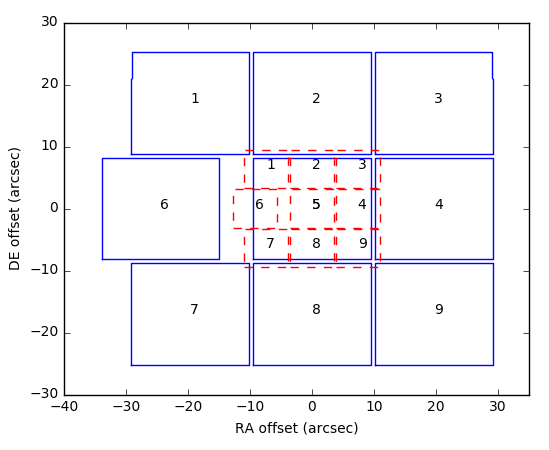
\includegraphics{images/fig3_fpa_footprint}}
    
    \caption{The footprints of the two imaging modes for MICADO. The wide-field mode (solid lines) has an on-sky footprint of $\sim 55\arcsec \times 50\arcsec$, while the zoom mode (dashed lines) has an on-sky footprint of $\sim 21\arcsec \times 19\arcsec$. The H4RG will only be 3-side buttable due to the placement of the read-out electronics, the result of which is the extended gap between chips~5 and~6 in the middle row.}
    
    \label{fig:fpa_footprint}
    
\end{figure}


\paragraph{Electronic noise:} \citet{nghxrg} created the python package NGHxRG\footnote{\url{http://jwst.nasa.gov/resources/nghxrg.tar.gz}} to simulate read noise frames for the HAWAII-2RG detectors used in the JWST NIRSpec instrument \citep{nirspec}. SimCADO uses this package to create noise frames for the HAWAII-4RG detector series. Included in the noise frames are: white (read) noise, residual bias drifts, pink $1/f$ noise and alternating column noise. Picture frame noise can also be included. However, as there are not yet any estimates for the MICADO detector array, SimCADO bases its picture frame noise on the default file provided by the NGHxRG package. The default parameters used when generating the noise frames are given in default configuration file in Appendix~\ref{appendix:micado_config}.


\paragraph{Detector gaps:} In its base configuration, the MICADO detector plane will consist of 9~H4RG detectors, each covering slightly more than $16\arcsec\times 16\arcsec$ on sky. Because of the read-out electronics, each chip will only be 3-side buttable, meaning that one of the eight outer chips must be placed further from the central chip than its counterparts. This can be seen in the on-sky footprints of the zoom and wide-field modes in Fig.~\ref{fig:fpa_footprint}. SimCADO contains configuration files detailing the positions of the detector chips for each of these base modes. 
% Due to the way SimCADO was built, any configuration of detectors is possible as long as the user specifies the centre of the chips relative to the centre of the focal plane array (in mm), the pixel size (in mm) and field of view and the pixel-dimensions of the chips. This feature is also useful for simulating the windowed read-out functionality of the H4RG chips.

\paragraph{Linearity, Saturation, Persistence and Cross-Talk:} Because detailed data on the H4RG chips are not yet publicly available, we have assumed that they will have a similar performance to the H2RG chips which are found in many current NIR instruments (e.g.~VLT/HAWK-I, JWST/NIRSpec). The data for the linearity curve and saturation limits have therefore been taken from the HAWK-I detector array. As persistence and pixel cross-talk are more complex to model, SimCADO does not currently simulate these two effects. We plan to implement them in a later version of SimCADO.

\paragraph{Read-out schemes:} SimCADO currently has two functions for reading out the chips on the detector array: ``non-destructive'' and ``super-fast''. The non-destructive mode mimics the functionality of the HAWAII-4RG chips, which allows the user to measure the pixel values without actually destroying the content of the pixels. This mode allows any non-destructive read-out scheme to be implemented, including the commonly used Fowler, double-correlated or up-the-ramp schemes. However, this mode is not the default and the scheme must be defined by the user.

For exposure times longer than the shortest exposure time for MICADO ($2.6\,\mathrm{s}$), observations will be background limited. Thus it is superfluous to calculate the read noise of each frame. Instead, by default, SimCADO uses a so-called ``super-fast'' read-out function. The ``super-fast'' function does not read out a series of single exposures every 2.6\,s, rather it creates a single read-out with an exposure time equal to the duration of the full observations (i.e. \verb+EXPTIME = NOBS*DIT+). Shot noise in the image scales as the square root of the total observation time. It is no surprise that the super-fast mode is NOBS times faster than the non-destructive read-out mode. For observations using the super-fast function which are greater than $\sim 10$\,minutes, we recommend ``turning off'' SimCADO's detector linearity functionality so that the signal increases linearly with exposure time over the full duration of the observation. In future releases this will occur automatically based on the chosen mode.
%\footnote{It should be noted that regardless of the status of the detector linearity, there is still a hard limit of $2.14\cdot10^{9}$ photons per pixel set by numpy's ``poisson'' function. Larger values raise an error message. Hence all pixel values above $2.14\cdot 10^{9}$ are capped so that shot noise can still be applied to the image.}

%\subsection{On whom does SimCADO depend for the data}

%Because SimCADO is an IDS, the package relies on data generated by other working groups that describe the optical effects present in the system which SimCADO simulates. As the development of MICADO is still a work in progress, we are continually updating the internal data sets as the new data becomes available. 

% While all data is equal in the eyes of its makers, some data sets are more equal than others. Data sets can be classified by their maturity and their volatility. Here mature means that the effect is well characterised and there is no new or on-going development on that aspect of the optical train. Volatility refers to small changes in the optical element resulting in large changes in flux distribution or transmission in the focal plane. Critical data is that which is both immature and volatile. It is the critical data sets which we keep an eye on and try to update as soon as new results are available. Table \ref{tbl:critical_data} gives a brief list of the most critical data sets in SimCADO.

%{\bf Put in a table here detailing the critical data sets}
% PSF, Optical designs of ELT, MAORY and MICADO and transmission and emission coefficients